% For instructions,
\documentclass[reprint, amsmath, amssymb, aps, onecolumn]{revtex4-2}

%\usepackage[norsk]{babel}
%Uncomment this if you want to write in Norwegian

\usepackage{graphicx}% Include figure files
\usepackage{dcolumn}% Align table columns on decimal point
\usepackage{bm}% bold math
\usepackage{hyperref}% add hypertext capabilities
\usepackage{booktabs}
\usepackage{float}
\usepackage{siunitx}
\usepackage{subcaption}
\usepackage{xcolor}
\usepackage{hyperref}
\hypersetup{
    colorlinks=true,
    linkcolor={red!60!black},
    filecolor=magenta,
    urlcolor=cyan,
    citecolor=blue!80!black
}

\usepackage[raggedright]{titlesec}
\usepackage{minted}

% \renewcommand{\vec}[1]{\mathbf{#1}} %ny definisjon av \vec så det blir bold face i stedet for vector-pil.
\newcommand{\LLRA}{\\[-1.3\baselineskip] $\Longleftrightarrow$ \\[-1.3\baselineskip]}

% \newcommand{\up}{\uparrow}
% \newcommand{\down}{\downarrow}
% \newcommand{\up}{\frac{1}{2}}
% \newcommand{\down}{-\frac{1}{2}}


% \newcommand{\dd}[4]{\left(\frac{\partial #1}{\partial #2}_{#3,#4}\right)
\newcommand{\dd}[3]{\left(\frac{\partial #1}{\partial #2}\right)_{#3}}


% \usepackage{braket}
% \usepackage{minted}

\begin{document}
\title{FYS4130 - Oblig 1}


\author{Mikkel Metzsch Jensen}

\date{\today}
\maketitle
%
\section*{Problem 1}
\noindent We have the following mapping by the black box.
\begin{align*}
  T, V, \mu \rightarrow P, N.
\end{align*}
Thus we are able to calculate numerical derivatives of $P$ and $N$ with respect to $T$, $V$ and $\mu$ respectively (with the others held constant). When considering the expression for the compressibility at consatant $T$ and $N$
\begin{align*}
  \kappa_T = -\frac{1}{V} \dd{V}{P}{T,N},
\end{align*}
we see that a natural starting point might by the reciprocal of the derivative $\partial V/\partial P$. Then it just remains to be manipulated such that we can interchange the constant $N$ with at constant $\mu$. We get
\begin{align}
  - \frac{1}{\kappa_T V} = \dd{P}{V}{T,N} = \frac{\partial (P,T,N)}{\partial (V,T,\mu)} \frac{\partial (V,T,\mu)}{\partial (V,T,N)} = \frac{\partial (P,N,T)}{\partial (V,\mu,T)} \dd{\mu}{N}{V,T}, \label{eq:prob1_start}
\end{align}
where we used the jacobian formulation and the chain rule to introduce $\mu$. The last term of eq.~\eqref{eq:prob1_start} can be calculated with the black box as the reciprocal of $\partial N / \partial \mu$ with constant $V$ and $T$. For the first term we can write out the jacobian
\begin{align*}
  \frac{\partial (P,N,T)}{\partial (V,\mu,T)} = \dd{P}{V}{\mu,T} \dd{N}{\mu}{V,T} - \dd{N}{V}{\mu,T}\dd{P}{\mu}{V,T}.
\end{align*}
We see immediately that all the derivatives act on variables $P$ or $N$, which are outputs of the black box, with respect to or held constant the variables $T, V, \mu$, which are inputs of the black box. Hence we have reached an expression that is compatible with the black box. However to simplify the expression slightly we can use the idendity
\begin{align*}
  \dd{N}{V}{\mu,T} = \dd{P}{\mu}{V,T},
\end{align*}
such that we get
\begin{align*}
  \frac{\partial (P,N,T)}{\partial (V,\mu,T)} = \dd{P}{V}{\mu,T} \dd{N}{\mu}{V,T} - \dd{P}{\mu}{V,T}^2.
\end{align*}
When gathering all the previous equations into eq.~\eqref{eq:prob1_start} we arrive at the final expression
\begin{align*}
  - \frac{1}{\kappa_T V} =  \frac{\dd{P}{V}{\mu,T} \dd{N}{\mu}{V,T} - \dd{P}{\mu}{V,T}^2}{\dd{N}{\mu}{V,T}}
\end{align*}
\LLRA
\begin{align*}
  \kappa_T = -\frac{1}{V} \frac{\dd{N}{\mu}{V,T}}{\dd{P}{V}{\mu,T} \dd{N}{\mu}{V,T} - \dd{P}{\mu}{V,T}^2}.
\end{align*}
The above expression contains only derivatives with can be elvaluated numerically using the black box
%
%%
%%%
%%
%
\section*{Problem 2}

\noindent For this problem it is usefull to write down the infinitesimal expression of the fundamental relations
\begin{align}
  dU &= TdS - PdV + \mu dN \label{eq:dU}, \\
  dG &= -SdT + VdP + \mu dN \label{eq:dG}.
\end{align}
We start by introducing $\partial(P,T,N)$ using the chain rule on the jacobian formulation
\begin{align}
  \dd{U}{P}{G,N} &= \frac{\partial (U, G, N)}{\partial (P,T,N)} \frac{\partial (P,T,N)}{\partial (P,G,N)} = \frac{\partial (U, G, N)}{\partial (P,T,N)} \dd{G}{T}{P,N}^{-1}. \label{eq:start}
\end{align}
From eq.~\eqref{eq:dG} we see that the last term of eq.~\eqref{eq:start} is $(-S)^{-1}$. We can write out the Jacobian of the first term as
\begin{align}
  \frac{\partial (U, G, N)}{\partial (P,T,N)} = \dd{U}{P}{T,N}\dd{G}{T}{P,N} - \dd{G}{P}{T,N}\dd{U}{T}{P,N}. \label{eq:jac}
\end{align}
Again using eq.~\eqref{eq:dG} we find
\begin{align*}
  \dd{G}{T}{P,N} = -S, \qquad \dd{G}{P}{T,N} = V.
\end{align*}
For the remaning terms we write out the derivatives using eq.~\eqref{eq:dU}.
\begin{align}
  \dd{U}{P}{T,N} &= T\dd{S}{P}{T,N} - P\dd{V}{P}{T,N} = -T\dd{V}{T}{P,N} - P\dd{V}{P}{T,N}, \label{eq:dd1} \\
  \dd{U}{T}{P,N} &= T\dd{S}{T}{P,N} - P\dd{V}{T}{P,N},
\end{align}
where we used the idendity $\dd{S}{P}{T,N} = -\dd{V}{T}{P,N}$ for eq.~\eqref{eq:dd1}. By using the standard quanties
\begin{align*}
  \alpha = \frac{1}{V}\dd{V}{T}{P,N}, \qquad
  \kappa_T = -\frac{1}{V}\dd{V}{P}{T,N}, \qquad
  c_P = \frac{T}{N}\dd{S}{T}{P,N},
\end{align*}
eq.~\eqref{eq:jac} can be written as
\begin{align*}
  \frac{\partial (U, G, N)}{\partial (P,T,N)} &= (-T\alpha V + P\kappa_T V)(-S) - V(c_P N - P \alpha V).
\end{align*}
Inserting this back into eq.~\eqref{eq:start} we get
\begin{align*}
  \dd{U}{P}{G,N} = \frac{(-T\alpha V + P\kappa_T V)(-S) - V(c_P N - P \alpha V)}{-S} = V\frac{(P\kappa_T -T\alpha)S + (c_P N - P \alpha V)}{S},
\end{align*}
such that the final answer is simply found as the reciprocal
\begin{align*}
  \dd{P}{U}{G,N} = \frac{1}{V}\frac{S}{(P\kappa_T -T\alpha )S + (Nc_P - P \alpha V)}.
\end{align*}
\clearpage
%
%%
%%%
%%
%
\section*{Problem 3}
\subsection*{a)}
\noindent We have Helmholtz free energy
\begin{align*}
  F = T\Big[ N_{x} \ln \left(\alpha l b^{2} \frac{N_{x}}{V}\right)+N_{y} \ln \left(\alpha b^{2} l \frac{N_{y}}{V}\right) + N_{z} \ln \left(\alpha b^{2} l \frac{N_{z}}{V}\right)+\gamma l b^{2} \frac{N_{x} N_{y}+N_{y} N_{z}+N_{z} N_{x}}{V}\Big],
\end{align*}
where we are going to use $\alpha = 1$, $\gamma = 10$ and $T = 1$ throughout problem 3. By defining the dimensionless volume $\tilde{V} = V/lb$ we get
\begin{align}
  \frac{F}{T} = &N_x \ln{\left(\alpha \frac{N_x}{\tilde{V}}\right)} + N_y \ln{\left(\alpha \frac{N_y}{\tilde{V}}\right)} + N_z \ln{\left(\alpha \frac{N_z}{\tilde{V}}\right)} + \gamma \frac{N_xN_y + N_yN_z + N_zN_x}{\tilde{V}}. \label{eq:3a}
\end{align}
%
%%
%
\subsection*{b)}
\noindent A numerical approach for this problem is to evaluate Helmholtz free energy $F$ for all possible configurations of orientations $\{N_x, N_y, N_z\}$ which sums to $N$. We can use eq.~\eqref{eq:3a} with reduced volumes, where the right hand side will be equal to $F$ for our choice $T = 1$. The equilibrium Helmholtz free energy $F_{eq}$ can then be calculated as the minimum $F$ among the computed values. Note that any permutation of a configuration will yield the same value of $F$ and thus we have at least three valid configurations for $F_{eq}$. For practical reasons I will choose the permutation where $N_x$, $N_y$ and $N_z$ appears in rising order. \par
Following the approach outlined above we can compute $F_{eq}$ as a function of $N$ or $\tilde{n} = N/\tilde{V}$. The corresponding equlibrium pressure can be calculated as
\begin{align*}
  P_{eq} = -\dd{F}{V}{T,N} \Big|_{\{N_{eq}\}} = T\left(\frac{N_x}{V} + \frac{N_y}{V} + \frac{N_z}{V} + \gamma \frac{N_xN_y + N_yN_z + N_zN_x}{\tilde{V^2}}\right)\Big|_{\{N_{eq}\}},
\end{align*}
where $\{N_{eq}\}$ denotes that we use an equlibrium configuration. Regarding the stability of the system we can use the energy minimum principle
\begin{align}
  \left(\frac{\partial^2 F}{\partial N^2}\right)_{T,V} \ge 0, \label{eq:stability}
\end{align}
which holds with respect to any extensive variable \cite{Svendsen}( chapter 15.2). By calculating the double derivative from eq.~\eqref{eq:stability} we can highlight whenever a phase transistion might accour. The code for the numerical calculations is shown in appendix \ref{sec:code_3b}. The results of the numerical calcualtions are shown in figure \ref{fig:res1}

\begin{figure}[H]
     \centering
     \begin{subfigure}[b]{0.49\textwidth}
         \centering
         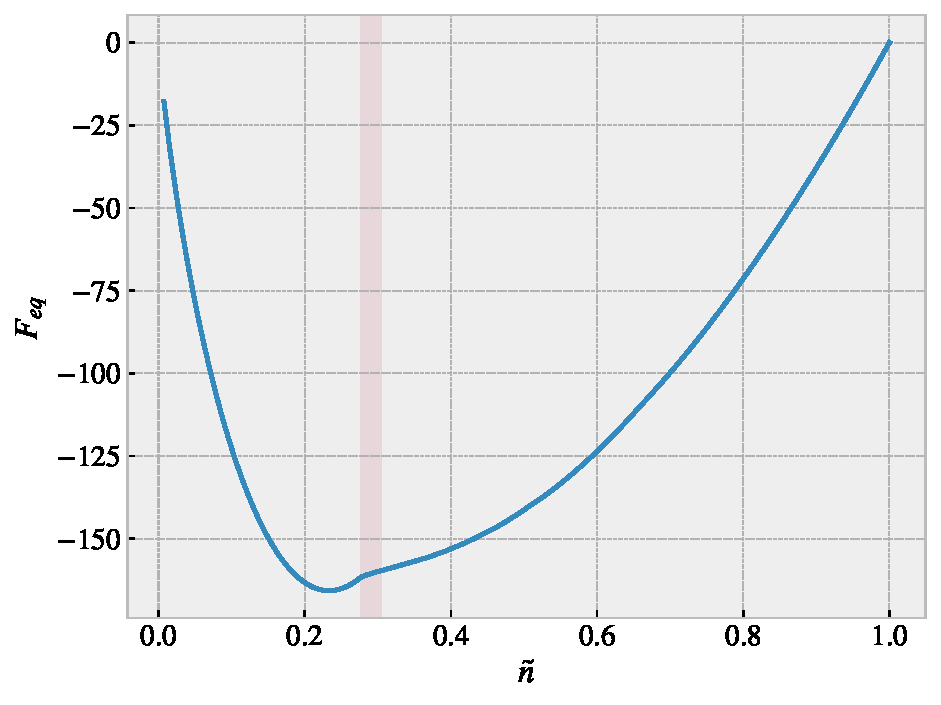
\includegraphics[width=\textwidth]{figures/Feq.pdf}
         \caption{Helmholtz free energy at equilibrium as a function of the reduced density.}
         \label{fig:Feq}
     \end{subfigure}
     \hfill
     \centering
     \begin{subfigure}[b]{0.49\textwidth}
         \centering
         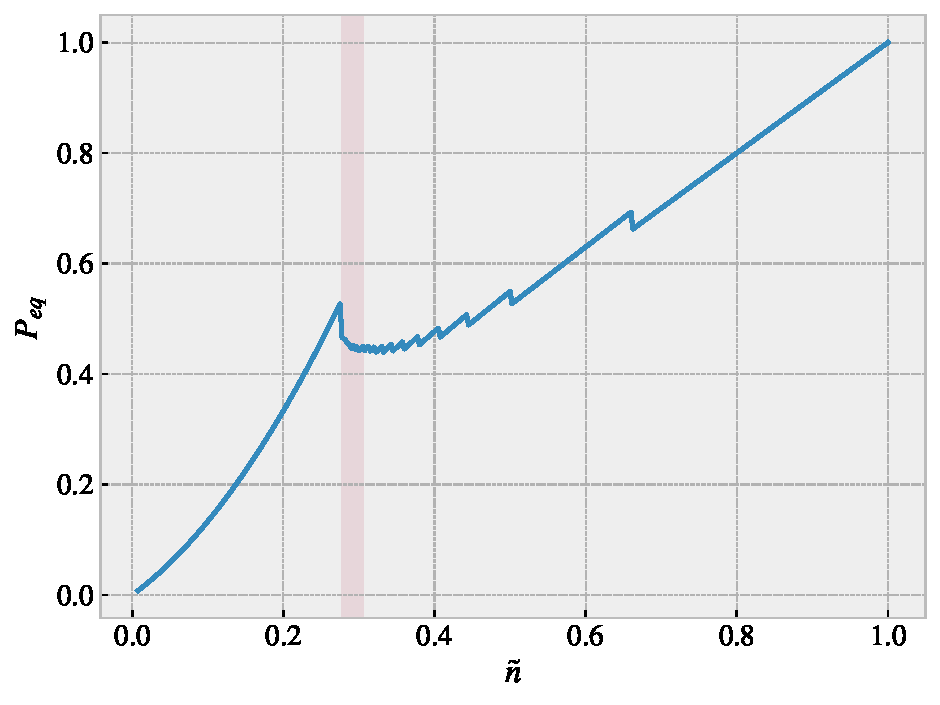
\includegraphics[width=\textwidth]{figures/Peq.pdf}
         \caption{The pressure at equlibrium as a function of the reduced density.}
         \label{fig:Peq}
     \end{subfigure}
     \hfill
     \centering
     \begin{subfigure}[b]{0.49\textwidth}
         \centering
         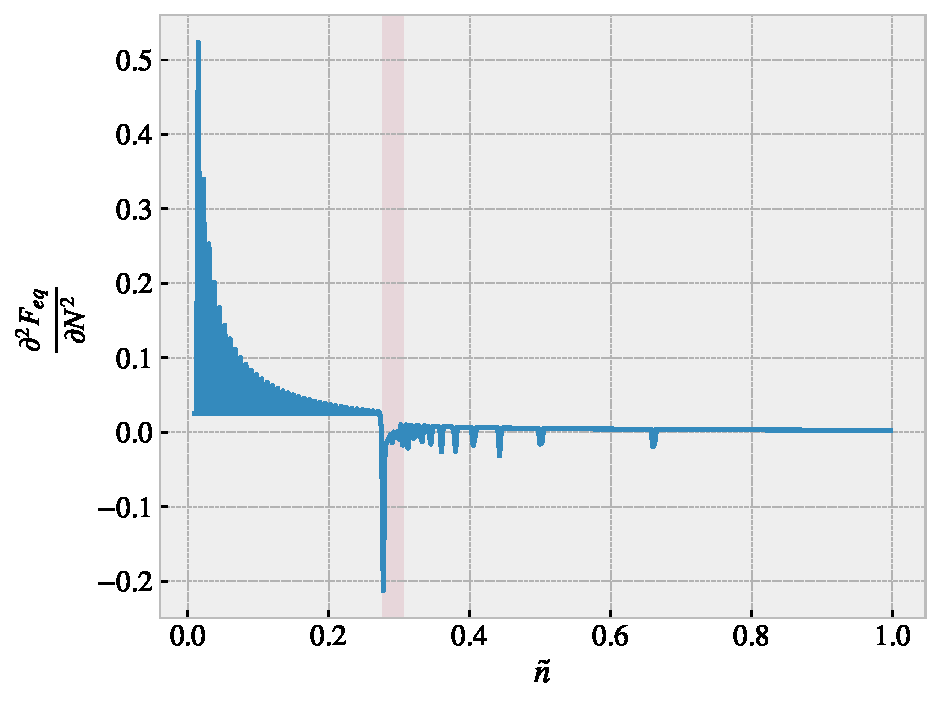
\includegraphics[width=\textwidth]{figures/ddFddN.pdf}
         \caption{Evaluation of the stability critera in eq.~\eqref{eq:stability} where negative values indicates instability.}
         \label{fig:ddFddN}
     \end{subfigure}
     \hfill
     \centering
     \begin{subfigure}[b]{0.49\textwidth}
         \centering
         \includegraphics[width=\textwidth]{figures/rod_conf.pdf}
         \caption{The rod configuration denoted as the number of rods pointing in $x$, $y$ and $z$ direction respectively. The configuration is permuted such that $N_x, N_y, N_z$ appears in increasing order.}
         \label{fig:rod_conf}
     \end{subfigure}
     \caption{Numerical results when calculating the equlibrium Helmholtz free energy for increasing reduced density $\tilde{n} = N/\tilde{V}$. Settings used:     $\alpha = 1$, $\gamma = 10$, $T = 1$, $V = 400$. The red domain, $p \in [0.2275, 0.3050]$, is the estimated area for coexsistence of phases which marks occurrence of phase transistions. This is computed as the longest continous domain for which the derivative in figure \ref{fig:ddFddN} takes a negative value.}
     \label{fig:res1}
\end{figure}
From the results in figure \ref{fig:res1} we observe a phase transistion from $n = 0.2275$ to $n \approx 0.3050$ where the double derivative $\partial F_{eq} / \partial N^2$ takes a negative value. The last bound should be taken more loosely as the double derivative $\partial^2 F/\partial N^2$ fluctuates such that it does not stay strictly positive after bouncing back from the negative values. This can be interpretated as the system being somewhat unstable in the new phase. However by this estimated bounds, the domain in beetween (red area on figure \ref{fig:res1}) marks the domain for coexsistence of phases. At phase transistion the pressure undergoes a seemingly discontinuous change where it drops in value. After the transistion it picks up an increasing trend again. However it shows a saw tooth pattern, which seems to be syncronized with $N_x$ and $N_y$ droping one integer in value each. For the configuration we see that before the phase transistion the rods is equally distributed in the three possible directions (as good as possible at least). After the phase tranasistion the system favors a majority of the rods pointing in the same direction.
%
%%
%
\subsection*{c)}
\noindent We follow a similar approach as in subquestion b), however now we keep $N$ constant and vary $\tilde{V}$. We calculate the Gibbs free energy at equlibrium as $G_{eq} = F_{eq} + PV$. The results is easiest to interpret for a small number of particles and hence we use $N = 5$. Regarding the stability we can use a similar stability condition as in subquestion b) as
\begin{align}
    \left(\frac{\partial^2 F}{\partial V^2}\right)_{T,V} = -\dd{P}{V}{T,N} \ge 0, \label{eq:stability2}
\end{align}
and thus we calculate $\partial P / \partial V$ to check for unstability. The code for the numerical calculations is shown in appendix \ref{sec:code_3c}. The numerical results is shown in figure \ref{fig:res2}


\begin{figure}[H]
     \centering
     \begin{subfigure}[b]{0.49\textwidth}
         \centering
         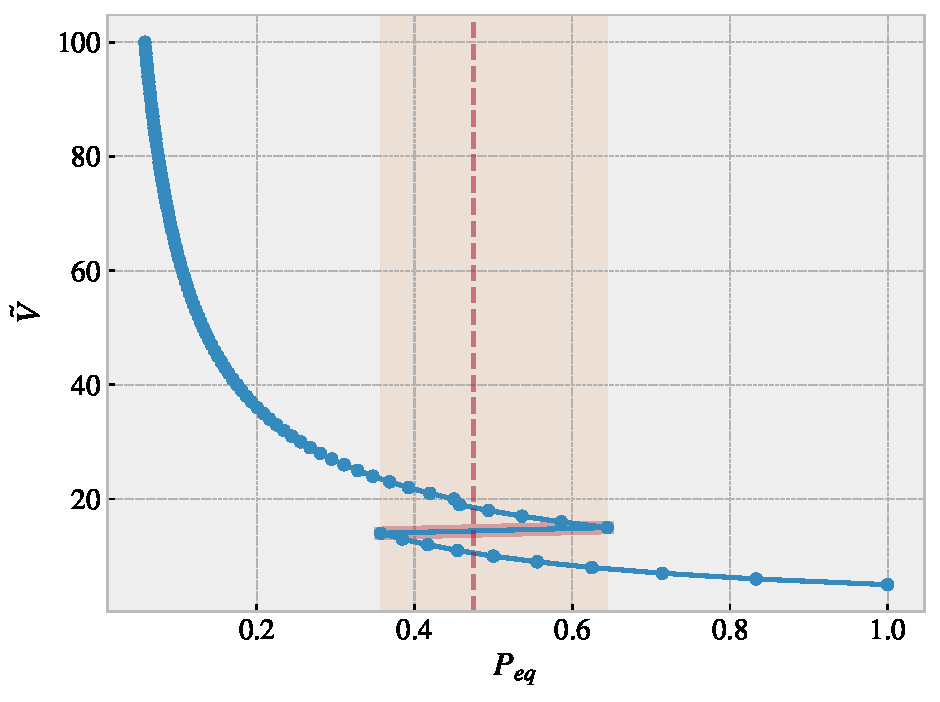
\includegraphics[width=\textwidth]{figures/VeqP.pdf}
         \caption{Reduced volume as a function of pressure at equlibrium}
         \label{fig:VeqP}
     \end{subfigure}
     \hfill
     \centering
     \begin{subfigure}[b]{0.49\textwidth}
         \centering
         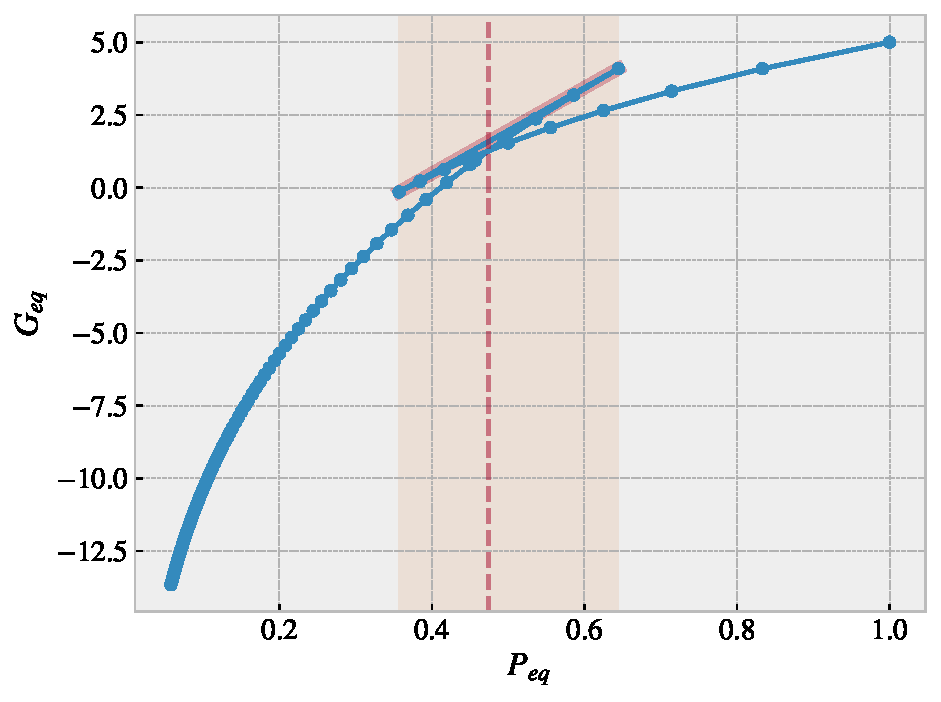
\includegraphics[width=\textwidth]{figures/Geq.pdf}
         \caption{Gibbs free energy as a function of pressure at equlibrium }
         \label{fig:Geq}
     \end{subfigure}
     \begin{subfigure}[b]{0.49\textwidth}
         \centering
         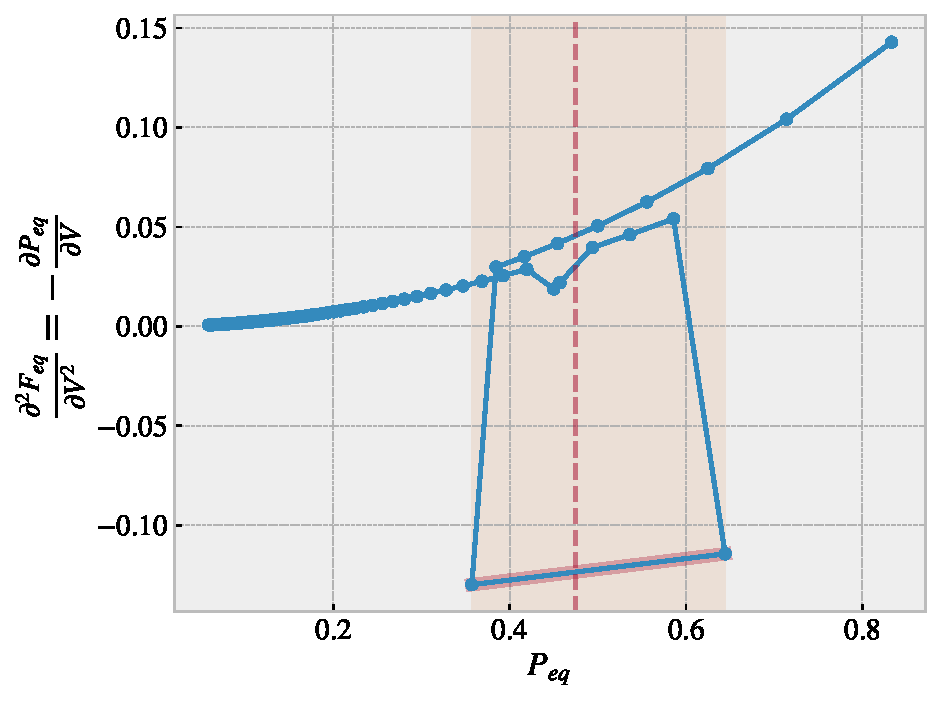
\includegraphics[width=\textwidth]{figures/ddFddV.pdf}
         \caption{Evaluation of the stability critera in eq.~\eqref{eq:stability2} where a negative value indicates unstability.}
         \label{fig:dPdV}
     \end{subfigure}
     \begin{subfigure}[b]{0.49\textwidth}
         \centering
         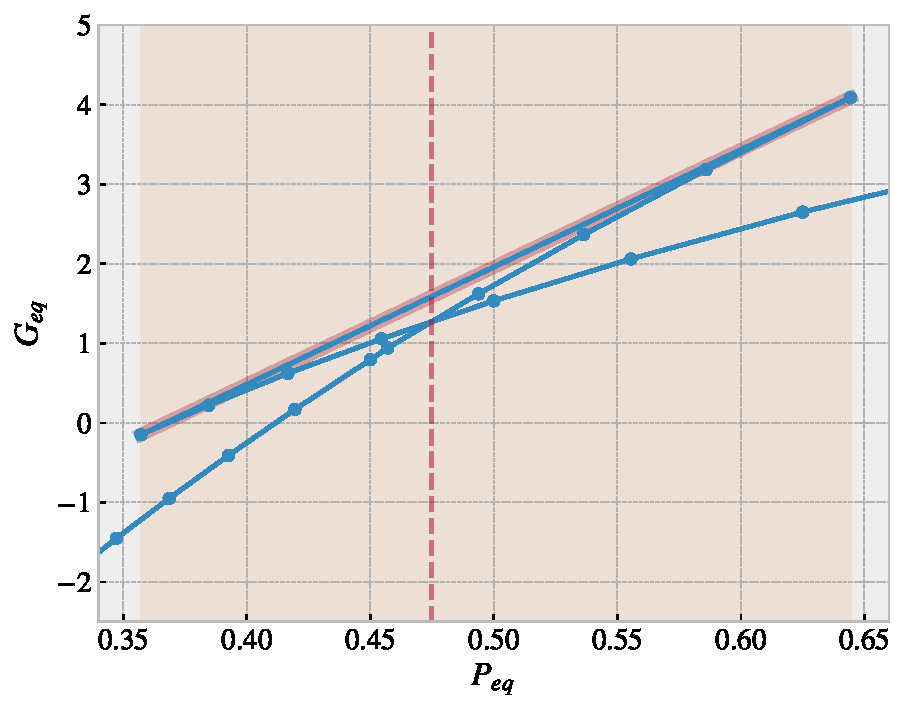
\includegraphics[width=\textwidth]{figures/Geq_zoom.pdf}
         \caption{figure \ref{fig:Geq} zoomed in.}
         \label{fig:Geq_zoom}
     \end{subfigure}
     \caption{Numerical results when calculating the equlibrium Gibbs free energy for increasing reduced volume. Settings used: $\alpha = 1$, $\gamma = 10$, $T = 1$, $N = 5$. The orange domain, $p \in [0.3571, 0.6444]$, marks a violation of the stability criteria from eq.~\eqref{eq:stability2}, while the red highlight marks the actual path where the criteria is violated. The vertical red dotted line, $p = 0.4748$ is manually placed at the self intersection in figure \ref{fig:Geq}.}
     \label{fig:res2}
\end{figure}

From the results in figure \ref{fig:res2} we see a behvaiour that resembles the phase tranasistion of the Van der Waals-gas \cite{Svendsen}(figure 17.2 and 17.3). From this we expect a phase transistion to accour at the red dotted line in figure \ref{fig:Geq} at $p = 0.4748$ while the orange domain in general marks the unstable region. Looking at figure \ref{fig:Geq} the uppermost red highlighted path is unstable to small pertubations since $\partial F^2/\partial V^2 < 0$ on this path. The path just below that is metastable since it is stable to small pertubations ($\partial F^2/\partial V^2 \ge 0$), but eventually it will drop to the true equlibrium state (the lowermost path) which lowers the gibbs free energy. When increasing the pressure towards the critical point marked by the red dotted line the phase transistion will result in a discontinuous change in the volume.
%
%%
%%%
%%
%
\section*{Problem 4}
\subsection*{a)}
\noindent With $N$ particles and $N_+$ of them having energy $+J$, the number of different microstates is a $N$ choose $N_+$ problem. This is described by the binomial coefficient
\begin{align}
  \begin{pmatrix} N \\ N_+ \end{pmatrix} = \frac{N!}{N_+!(N-N_+)!}. \label{eq:omega}
\end{align}
%
%%
%
\subsection*{b)}
\noindent The entropy can be calculated using the Boltzmann definition $S = k_B \ln{\Omega}$, where $\Omega$ is the number of microstates corresponding to eq.~\eqref{eq:omega}. For large $N$ we can use the stirling approximation $\ln{N!} = N\ln{N} - N$ such that we get
\begin{align}
  \frac{S}{k_B} = \ln{\left(\frac{N!}{N_+!(N-N_+)!} \right)} &= \ln{N!} - \ln{N_+!} - \ln{(N-N_+)!} \nonumber\\
  &= N\ln{N} - N -\big(N_+ \ln{N_+} - N_+\big) - \big((N-N_+)\ln{(N-N_+)} - (N - N_+)\big) \nonumber\\
  &= N\ln{\left(\frac{N}{N-N_+}\right)} +  N_+ \ln{\left(\frac{N-N_+}{N_+}\right)}. \label{eq:S1}
\end{align}
To reveal the relationship between $N_+$ and $T$ we first rewrite $E$ as $E = J(2N_+ - N)$, using $N = N_+ + N_-$. By using the definition of temperature we find
\begin{align*}
  \frac{1}{T} &= \dd{S}{U}{V,N} = \dd{S}{E}{N} = \frac{\partial S}{\partial N_+}\frac{\partial N_+}{\partial E} \\
  &= \frac{k_B}{2J}\left[N\frac{N-N_+}{N}\frac{N}{(N-N_+)^2} + \ln{\left(\frac{N-N_+}{N_+}\right)} + N_+ \frac{N_+}{N-N_+} \frac{-N}{N_+^2}  \right] \\
  &= \frac{k_B}{2J}\left[ \frac{N}{N-N_+} + \ln{\left(\frac{N-N_+}{N_+}\right)} - \frac{N}{N-N_+}\right] \\
  &= \frac{k_B}{2J} \ln{\left(\frac{N-N_+}{N_+}\right)}.
\end{align*}
\LLRA
\begin{align}
  \frac{N-N_+}{N_+} &= e^{2J\beta} \nonumber\\
  N_+ &= \frac{N}{e^{2J\beta} + 1}, \qquad \beta = \frac{1}{k_B T}. \label{eq:N_+}
\end{align}

Plugging eq.~\eqref{eq:N_+} back into eq.~\eqref{eq:omega} we get
\begin{align*}
  S &= k_BN\ln{\left(\frac{N}{N-\frac{N}{e^{2J\beta} + 1}}\right)} +  \frac{Nk_B}{e^{2J\beta} + 1} \ln{\left(\frac{N-\frac{N}{e^{2J\beta} + 1}}{\frac{N}{e^{2J\beta} + 1}}\right)} \\
  &=  Nk_B\ln{\left(\frac{e^{2J\beta} + 1}{e^{2J\beta}}\right)} + \frac{Nk_B}{e^{2J\beta} + 1} \ln{\left(e^{2J\beta}\right)} \\
  &=  Nk_B\ln{\left(1 + e^{-2J\beta}\right)} + Nk_B\frac{2J\beta}{e^{2J\beta} + 1} \\
  &=  Nk_B\left[\ln{(1 + e^{-2J\beta})}
 + \frac{2J\beta}{e^{2J\beta} + 1} \right]. \\
\end{align*}
%
%%
%
\subsection*{c)}
\noindent The heat capacity (with either constant volume or pressure) is defined as
\begin{align*}
  c = \frac{T}{N}\dd{S}{T}{N},
\end{align*}
and thus we get
\begin{align*}
  c &= \frac{T}{N}\frac{\partial S}{\partial \beta} \frac{\partial \beta}{\partial T} = -\frac{1}{k_B T N} \frac{\partial S}{\partial \beta} \\
  &= -\beta k_B \frac{\partial}{\partial \beta}\left[\ln{(1 + e^{-2J\beta})}
 + \frac{2J\beta}{e^{2J\beta} + 1} \right] \\
 &= -\beta k_B \left[-\frac{2Je^{-2j\beta}}{1 + e^{-2J\beta}} + \frac{2J(e^{2J\beta} + 1) - 4J^2\beta e^{2J\beta}}{(e^{2J\beta} + 1)^2} \right] \\
 &= -\beta k_B \left[-\frac{2J}{e^{2J\beta} + 1} + \frac{2J(e^{2J\beta} + 1) - 4J^2\beta e^{2J\beta}}{(e^{2J\beta} + 1)^2} \right] \\
  &= k_B \left( \frac{2J\beta}{e^{2J\beta} + 1} \right)^2 e^{2J\beta}.
\end{align*}
We can then inspect the temperature limits. \\
\\
$T \to 0 \Longleftrightarrow \beta \to \infty:$
\begin{align*}
   \lim_{\beta\to\infty} c &= \lim_{\beta\to\infty} \left[ k_B \left( \frac{2J\beta}{e^{2J\beta} + 1} \right)^2 e^{2J\beta} \right]\\
   &=  4J^2k_B \lim_{\beta\to\infty} \left[ \frac{\beta^2 e^{2J\beta}}{e^{4J\beta} + 1 + 2e^{2J\beta}} \right] \\
   &=  4J^2k_B \lim_{\beta\to\infty} \left[ \frac{\beta^2 }{e^{2J\beta} + e^{-2J\beta} + 2} \right] \\
   &\overset{L'H}=  4J^2k_B \lim_{\beta\to\infty} \left[ \frac{2\beta }{2Je^{2J\beta}  -2Je^{-2J\beta}} \right] \\
   &\overset{L'H}=  k_B \lim_{\beta\to\infty} \left[ \frac{2 }{e^{2J\beta} + e^{-2J\beta}} \right] = 0\\
\end{align*}
$T \to \infty \Longleftrightarrow \beta \to 0:$
\begin{align*}
  \lim_{\beta\to0} c &= \lim_{\beta\to0} \left[ k_B \left( \frac{2J\beta}{e^{2J\beta} + 1} \right)^2 e^{2J\beta} \right] = k_B \left(\frac{2J\cdot0}{2}\right)^2 = 0
\end{align*}
We find that the heat capcity goes towards zero for both $T\to0$ and $T\to\infty$.

\begin{thebibliography}{}
  \bibitem{Svendsen} Svendsen, Robert H., An introduction to Statistical Mechanics and Thermodynamics, Second edition 2020.
\end{thebibliography}
\clearpage


\appendix
\section{Code}
\subsection{Problem 3 b)}\label{sec:code_3b}

\begin{minted}[breaklines, breakautoindent=true]{python}
import numpy as np
import matplotlib.pyplot as plt
from plot_set import * # Plotting settings

alpha = 1
gamma = 10
def cal_F(N_arr, V, T):
    """ return F with repsect to configuration N_rr,
        temperature T and dimensionless volume V """
    sum = 0
    for N_ in N_arr[N_arr > 0]:
        sum += N_*np.log(alpha*N_/V)
    return T*(sum + gamma*(N_arr[0]*N_arr[1] + N_arr[1]*N_arr[2] + N_arr[2]*N_arr[0])/V)

def cal_P(N_arr, V, T):
    """ Calculate pressure with respect configuration N_rr
        dimensionless volume V and temperature T """
    Nx, Ny, Nz = N_arr
    P = T*(Nx/V + Ny/V + Nz/V + gamma*(Nx*Ny + Ny*Nz + Nz*Nx)/V**2)
    return P


def minimum_F(N, V, T):
    """ Go through all possible configurations and
        return minimum F with respect to number of particles N,
        dimensionless volume and temperature T """
    minF = 1e10
    N = int(N)
    state = np.zeros(3)
    trial_state = np.zeros(3)
    for Nx in range(N+1):
        for Ny in range(N-Nx+1):
            Nz = N - Nx - Ny
            trial_state[:] = (Nx, Ny, Nz)

            F = cal_F(trial_state, V, T)

            if F < minF:
                minF = F
                state[:] = trial_state[:]
    state.sort()
    return minF, state


def equil_states_N(N_start, N_end, V, T):
    """ Gather equlibrium F, P and configurations for
        increasing N for dimensionsless volume V and temperature T """
    N = np.linspace(N_start, N_end, N_end - N_start + 1)
    F = np.zeros(len(N))
    P = np.zeros(len(N))
    states = np.zeros((len(N), 3))
    for i in range(len(N)):
        F[i], states[i] = minimum_F(N[i], V, T)
        P[i] = cal_P(states[i], V, T)
        print(f'\rN = {int(N[i])}/{int(N[-1])}, state = {states[i]}', end='')
    print()

    ddFddN = double_derivative(N, F)
    dd_neg = np.argwhere(ddFddN < 0).ravel()
    phase_trans = [dd_neg[0]]
    for i in range(1, len(dd_neg)):
        if dd_neg[i] - dd_neg[i-1] > 2:
            break
        phase_trans.append(dd_neg[i])
    phase_trans = np.array(phase_trans)

    save = True
    n = N/V
    print(f'Estimated phase trans, n: {n[phase_trans][0]}, {n[phase_trans][-1]}')

    axis_label_size = 16
    plt.figure(num=0, dpi=80, facecolor='w', edgecolor='k')
    plt.plot(n, F)
    plot_area(n[phase_trans], plt.gca())
    plt.xlabel(r"$\tilde{n}$", fontsize = axis_label_size)
    plt.ylabel(r"$F_{eq}$", fontsize = axis_label_size)
    plt.tight_layout(pad=1.1, w_pad=0.7, h_pad=0.2)
    if save:
        plt.savefig("../article/figures/Feq.pdf", bbox_inches="tight")

    plt.figure(num=1, dpi=80, facecolor='w', edgecolor='k')
    plt.plot(n, P)
    plot_area(n[phase_trans], plt.gca())

    plt.xlabel(r"$\tilde{n}$", fontsize = axis_label_size)
    plt.ylabel(r"$P_{eq}$", fontsize = axis_label_size)
    plt.tight_layout(pad=1.1, w_pad=0.7, h_pad=0.2)
    if save:
        plt.savefig("../article/figures/Peq.pdf", bbox_inches="tight")

    plt.figure(num=2, dpi=80, facecolor='w', edgecolor='k')
    plt.plot(n, ddFddN)
    plot_area(n[phase_trans], plt.gca())
    plt.xlabel(r"$\tilde{n}$", fontsize = axis_label_size)
    plt.ylabel(r"$\frac{\partial^2 F_{eq}}{\partial N^2}$", fontsize = 20)
    plt.tight_layout(pad=1.1, w_pad=0.7, h_pad=0.2)
    if save:
        plt.savefig("../article/figures/ddFddN.pdf", bbox_inches="tight")

    plt.figure(num=3, dpi=80, facecolor='w', edgecolor='k')
    plt.plot(n, states[:,0], color = color_cycle(0), label = "# $N_x$")
    plt.plot(n, states[:,1], color = color_cycle(2), label = "# $N_y$")
    plt.plot(n, states[:,2], color = color_cycle(3), label = "# $N_z$")
    plot_area(n[phase_trans], plt.gca())
    plt.xlabel(r"$\tilde{n}$", fontsize= axis_label_size)
    plt.ylabel(r"Rod configuration", fontsize=14)
    plt.legend(fontsize = 13)

    plt.tight_layout(pad=1.1, w_pad=0.7, h_pad=0.2)
    if save:
        plt.savefig("../article/figures/Rod_conf.pdf", bbox_inches="tight")


    plt.show()


def plot_area(x, ax, color = color_cycle(1)):
    """ Shade x domain area with red color """
    ax = plt.gca()
    ylim = ax.get_ylim()
    plt.fill_between(x, ylim[0], ylim[1], alpha = 0.1, color = color)
    ax.set_ylim(ylim)

def double_derivative(x, y):
    """ Second order central finite difference """
    h = 1
    dd = np.zeros(len(x))
    dd[:] = np.nan
    for i in range(h, len(y)-h):
        dd[i] = (y[i+h] - 2*y[i] + y[i-h])/h**2

    return dd


if __name__ == "__main__":
    V = 400
    T = 1
    N_start = 3
    N_end = V
    equil_states_N(N_start, N_end, V, T)

\end{minted}

\clearpage
\subsection{Problem 3 c)}\label{sec:code_3c}
\begin{minted}[breaklines, breakautoindent=true]{python}
from prob3b import *

def equil_states_V(V_start, V_end, N, T):
    """ Gather equlibrium F, G, P and configurations for
        increasing V for number of particles N and temperature T """
    V = np.linspace(V_start, V_end, V_end - V_start + 1)
    F = np.zeros(len(V))
    G = np.zeros(len(V))
    P = np.zeros(len(V))
    states = np.zeros((len(V), 3))

    for i in range(len(V)):
        F[i], states[i] = minimum_F(N, V[i], T)
        P[i] = cal_P(states[i], V[i], T)
        G[i] = F[i] + P[i]*V[i]
        print(f'\r{i}/{len(V)}, V = {V[i]:.2f}, ngamma = {gamma*N/V[i]:.2f}, state = {states[i]}', end='')
    print()

    dPdV = single_derivative(V, P)
    ddFddV = -dPdV
    phase_trans = np.argwhere(ddFddV < 0).ravel()


    save = True
    axis_label_size = 16

    plt.figure(num=0, dpi=80, facecolor='w', edgecolor='k')
    plt.plot(P[phase_trans], V[phase_trans], linewidth = 6, alpha = 0.3, color = color_cycle(1))
    plt.plot(P, V, '-o', markersize = 5)
    plot_area(P[phase_trans], plt.gca(), color = color_cycle(4))
    plt.gca().axvline(0.474811, linestyle = '--', color = color_cycle(1), alpha = 0.5)

    plt.xlabel(r"$P_{eq}$", fontsize = axis_label_size)
    plt.ylabel(r"$\tilde{V}$", fontsize = axis_label_size)
    plt.tight_layout(pad=1.1, w_pad=0.7, h_pad=0.2)
    if save:
        plt.savefig("../article/figures/VeqP.pdf", bbox_inches="tight")

    plt.figure(num=1, dpi=80, facecolor='w', edgecolor='k')
    plt.plot(P[phase_trans], G[phase_trans], linewidth = 6, alpha = 0.3, color = color_cycle(1))
    plt.plot(P, G, '-o', markersize = 5)
    plot_area(P[phase_trans], plt.gca(), color = color_cycle(4))

    plt.gca().axvline(0.474811, linestyle = '--', color = color_cycle(1), alpha = 0.5)
    plt.xlabel(r"$P_{eq}$", fontsize = axis_label_size)
    plt.ylabel(r"$G_{eq}$", fontsize = axis_label_size)
    plt.tight_layout(pad=1.1, w_pad=0.7, h_pad=0.2)
    if save:
        plt.savefig("../article/figures/Geq.pdf", bbox_inches="tight")
    plt.xlim([0.34, 0.66])
    plt.ylim(-2.5, 5)
    if save:
        plt.savefig("../article/figures/Geq_zoom.pdf", bbox_inches="tight")


    plt.figure(num=2, dpi=80, facecolor='w', edgecolor='k')
    plt.plot(P[phase_trans], -dPdV[phase_trans], linewidth = 6, alpha = 0.3, color = color_cycle(1))
    plt.plot(P, ddFddV, '-o', markersize = 5)
    plt.gca().axvline(0.474811, linestyle = '--', color = color_cycle(1), alpha = 0.5)
    plot_area(P[phase_trans], plt.gca(), color = color_cycle(4))

    plt.xlabel(r"$P_{eq}$", fontsize = axis_label_size)
    plt.ylabel(r"$\frac{\partial^2 F_{eq}}{\partial V^2} = - \frac{\partial P_{eq}}{\partial V}$", fontsize = 20)
    plt.tight_layout(pad=1.1, w_pad=0.7, h_pad=0.2)
    if save:
        plt.savefig("../article/figures/ddFddV.pdf", bbox_inches="tight")

    plt.show()


def single_derivative(x, y):
    """ First order central finite difference """
    h = 1
    d = np.zeros(len(x))
    d[:] = np.nan
    for i in range(h, len(y)-h):
        d[i] = (y[i+h] -  y[i-h])/(2*h)

    return d


if __name__ == "__main__":
    N = 5
    V_start = N
    V_end = 100
    T = 1
    equil_states_V(V_start, V_end, N, T)
\end{minted}




\end{document}
